\documentclass{report}
\usepackage {mathtext}
\usepackage{amsmath}
\usepackage [russian] {babel}
\usepackage{caption}
\captionsetup[table]{position=t,justification=raggedleft,slc=off}
\setlength{\abovecaptionskip}{0pt}
\usepackage {geometry}
\usepackage {amssymb}
\usepackage{graphicx}
\geometry{margin=1in}
\title{Лабораторная работа №1.1.1. \\ Определение систематических и случайных погрешностей при измерении удельного сопротивления нихромовой проволоки}
\author{Павел Рудачихин \\ Б04-507}
\date{04.09.2025}
\begin {document}
	\maketitle{}
	\section* {Аннотация} 
	
	В работе проверяется закон Ома и измеряется удельное сопротивление тонкой нихромовой проволоки круглого сечения. Исследуются случайные и систематические погрешности проводимых измерений.
	
	\textbf{Цель работы:} измерить удельное сопротивление проволоки и вычислить систематические и случайные погрешности при использовании некоторых измерительных приборов.

	\textbf{В работе используются:} линейка, штангенциркуль, микрометр, отрезок нихромовой проволоки, амперметр, вольтметр, источник ЭДС, мост постоянного тока, реостат.
	
	\textbf{Методы:} 1) определение  углового  коэффициента  наклона  зависимости 
	напряжения на отрезке проволоки от тока через него; 2) измерение напряжения с помощью аналогового вольтметра и тока с помощью цифрового амперметра; 3) измерение сопротивления отрезка проволоки с помощью моста постоянного тока; 4) измерение геометрических размеров проволоки с помощью линейки, штангенциркуля и микрометра. 
	
		
	\section* {Теоретические сведения}
	
	Известно, что удельное сопротивление материала однородного проводника круглого сечения и постоянной толщины выражено:
	
	\begin{equation} 
		\rho = \frac{R}{l}\frac{\pi d^{2}}{4},
	\end{equation}
	где $R$ - сопротивление отрезка проволоки, $l$ - его длина, $d$ - диаметр проволоки.
	
	Сопротивление отрезка проволоки можно вычислить по закону Ома для участка цепи:
	\begin{equation}
		U = IR,
	\end{equation}
	где $U$ - напряжение на участке, $I$ - ток через него.
	
	\section*{Методика измерений}
	
	Диаметр проволоки может быть измерен напрямую штангенциркулем и микрометром, а длина отрезка - линейкой. Сопротивление отрезка проволоки измеряется косвенно. Подробно остановимся на описании экспериментальной установки для измерения тока и напряжения.
	
	\subsection*{Экспериментальная установка}
	
	Известно, что амперметр подключается последовательно измеряемому участку, а вольтметр - параллельно. Однако возможны два варианта взаимного положения амперметра (А) и вольтметра (V), представленные на рис.1, где $\mathcal{E}$ - источник ЭДС, $R$ - реостат, $R_{A}$ - внутреннее сопротивление амперметра, $R_{V}$ - вольтметра, $R_{\text{ПР}}$ - отрезок проволоки. 
	
	\begin{figure}[!h]
		\centering
		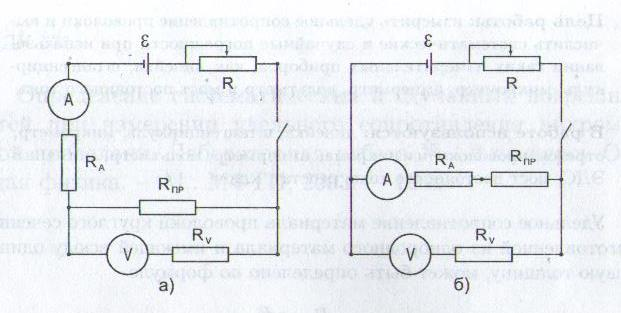
\includegraphics[width=0.5\linewidth]{s.jpg}
		\caption{Схемы установки}
		\label{fig:s}
	\end{figure}
	
	Различие между схемами определяется собственными сопротивлениями неидеальных приборов. Обозначим за $R$  истинное сопротивление отрезка проволоки, за $R^{*}$ - измеренное.
	
	\subsubsection* {Вариант 1 (рис. 1.а)}
	В реальности измеренное сопротивление будет эквивалентно параллельному соединению сопротивлений проволоки и вольтметра, поэтому:
	\begin{equation}
		R^{*} = \frac{R R_{V}}{R + R_{V}}
	\end{equation} 
	Преобразуем:
	\begin{equation}
		R = \frac{R^{*}R_{V}}{R_{V}-R^{*}} = \frac{R^{*}}{1-\frac{R^{*}}{R_{V}}} \approx R^{*}(1+\frac{R^{*}}{R_{V}})
	\end{equation} 
	
	\subsubsection* {Вариант 2 (рис. 1.б)}
	В реальности измеренное сопротивление будет эквивалентно последовательному соединению сопротивлений проволоки и амперметра, поэтому:
	\begin{equation}
		R^{*} = R + R_{A}
	\end{equation} 
	Преобразуем:
	\begin{equation}
		R =  R^{*}(1-\frac{R_{A}}{R^{*}})
	\end{equation}
	
	
	Таким образом, отклонение измеренного значения сопротивления $R^{*}$ от истинного $R$ определяется отношениями $\frac{R^{*}}{R_{V}}$ и $\frac{R_{A}}{R^{*}}$. Меньшее значение определит выбор схемы. 
	
	\section*{Используемое оборудование}
	
	\subsection*{Линейка}
	Погрешность линейки, исходя из цены деления, составляет $\Delta_{\text{Л}} = \pm 0,5$ мм. Но способ крепления проволоки к клеммам (а именно намотка нескольких витков и зажим) осложняет определение точки контакта, что вносит дополнительную погрешность. Оценим погрешность линейки в $\Delta_{\text{Л}} = \pm 2$ мм
	
	\subsection*{Штангенциркуль}
	Маркировка производителя: $\Delta_{\text{Ш}} = \pm 0,05$ мм
	
	\subsection*{Микрометр}
	Маркировка производителя: $\Delta_{М} = \pm 0,01$ мм
	
	\subsection*{Вольтметр}
	
	Основные характеристики вольтметра указаны в таблице 1.
	
	\begin{table}[!h]
		\centering
		\captionbox{Характеристики вольтметра}{
		\begin{tabular}{|l|c|}
			\hline
			Система & Магнитоэлектрическая \\
			\hline
			Класс точности  & 0,2 \\
			\hline
			Предел измерений  & 300 мВ \\
			\hline
			Число делений шкалы  & 150 \\
			\hline
			Цена делений  & 2 мВ/дел \\
			\hline
			Чувствительность  & 500 дел/В \\
			\hline
			Абсолютная погрешность  & 0,6 мВ \\
			\hline
			Внутреннее сопротивление  & 2 кОм \\
			\hline
		\end{tabular}}
	\end{table}
	
	Заметим, что цена деления 2 мВ, а погрешность, определённая по классу точности меньше: 0,6 мВ. Шкала не позволяет снять показания с погрешностью 0,6 мВ, поэтому будем пользоваться погрешностью, равной половине цены деления: $\pm 1$ мВ.
	
	\subsection*{Амперметр}
		
	Основные характеристики вольтметра указаны в таблице 2.
	
	\begin{table}[!h]
		\centering
		\captionbox{Характеристики амперметра}{
		\begin{tabular}{|l|c|}
			\hline
			Система & Цифровая \\
			\hline
			Предел измерений  & 2 А \\
			\hline
			Разрядность  & 5 единиц \\
			\hline
			Внутреннее сопротивление  & 1,2 Ом \\
			\hline
		\end{tabular}}
	\end{table}
	
	Показания снимались с точностью до десятых долей мА, поэтому можно оценить $\Delta_{A} = 0,1$ мА
	
	\subsection*{Мост постоянного тока Р4833}
	
	Основные характеристики моста постоянного тока указаны в таблице 3.
	
	\begin{table}[!h]
		\centering
		\captionbox{Характеристики моста постоянного тока}{
		\begin{tabular}{|l|c|}
			\hline
			Класс точности  & 0,1 \\
			\hline
			Предел измерений  & 10 Ом \\
			\hline
			Абсолютная погрешность  & 0,01 Ом \\
			\hline
		\end{tabular}}
	\end{table}
	
	\subsection*{Анализ влияния погрешностей}
	Для измерения длины $l$ возможно использование исключительно линейки. Для измерения диаметра $d$ следует использовать микрометр, т.к его погрешность меньше, чем у штангенциркуля.
	
	По формулам (4) и (6) оценим поправки для двух схем, приняв $R^{*} = 5$ Ом:
	
	$\frac{R^{*}}{R_{V}} = 0,0025$
	
	$\frac{R_{A}}{R^{*}} = 0,24$
	
	Очевидно, следует выбрать первый вариант схемы.
	
	\section*{Результаты измерений}
	
	Результаты всех измерений представлены в таблицах 4, 5 и 6.
	
	\begin{table}[!h]
		\centering
		\captionbox{Измерение диаметра проволоки}{
		\begin{tabular}{|r|rrrrrrrrrr|}
			\hline
			Штангенциркулем (мм) & 0,30  & 0,30  & 0,30  & 0,35  & 0,30  & 0,35  & 0,35  & 0,30  & 0,30  & 0,30 \\
			\hline
			Микрометром (мм)&0,31  & 0,30  & 0,30  & 0,30  & 0,30  & 0,29  & 0,29  & 0,30  & 0,30  & 0,29 \\
			\hline
		\end{tabular}}
	\end{table}
	
	\begin{table}[!h]
		\centering
		\captionbox{Измерение тока и напряжения}{
		\begin{tabular}{|ccc|}
			\hline
			 & l = 50 см& \\
			V, дел & V, мВ&I, мА \\
			\hline
			65    & 130   & 25,7 \\
			70    & 140   & 27,7 \\
			80    & 160   & 31,7 \\
			95    & 190   & 37,5 \\
			115   & 230   & 45,2 \\
			105   & 210   & 41,4 \\
			90    & 180   & 35,3 \\
			75    & 150   & 29,5 \\
			72    & 144   & 28,4 \\
			63    & 126   & 24,7 \\
			\hline
		\end{tabular}
		\begin{tabular}{|ccc|}
			\hline
			& l = 30 см& \\
			V, дел & V, мВ&I, мА \\
			\hline
			65    & 130   & 42,2 \\
			70    & 140   & 45,4 \\
			85    & 170   & 55,3 \\
			95    & 190   & 62,0 \\
			100   & 200   & 65,3 \\
			80    & 160   & 52,0 \\
			60    & 120   & 39,3 \\
			50    & 100   & 32,7 \\
			45    & 90    & 29,3 \\
			40    & 80    & 26,0 \\
			\hline
		\end{tabular}
		\begin{tabular}{|ccc|}
			\hline
			& l = 20 см& \\
			V, дел & V, мВ&I, мА \\
			\hline
			65    & 130 & 63,7 \\
			70    & 140 & 68,1 \\
			90    & 180 & 87,7 \\
			115   & 230 & 111,9 \\
			130   & 260 & 126,4 \\
			99    & 198 & 96,9 \\
			80    & 160 & 77,8 \\
			60    & 120 & 58,2 \\
			50    & 100 & 48,5 \\
			30    & 60  & 29,2 \\
			\hline
		\end{tabular}}
	\end{table}
	
	\begin{table}[!h]
		\centering
		\captionbox{Измерение сопротивления на мосте постоянного тока}{
		\begin{tabular}{|r|ccc|}
			\hline
			Длина, см & 50 & 30 & 20 \\
			\hline
			Сопротивление, Ом & 5,0462 & 3,0431 & 2,0481 \\
			\hline
		\end{tabular}}
	\end{table}
	
	\section*{Обработка результатов}
	\subsection*{Длина отрезка проволоки}
	
	В работе исследовались три отрезка проволоки, длины которых были измерены линейкой и равны соответственно:
	
	\begin{center}
		$l_{1} = (500 \pm 2)$ мм
		
		$l_{2} = (300 \pm 2)$ мм
		
		$l_{3} = (200 \pm 2)$ мм
	\end{center}
	
	
	\subsection*{Диаметр и поперечное сечение проволоки}
	
	При измерении штангенциркулем получено следующее значение диаметра:
	
	\begin{equation}
		\bar{d_{1}}= \frac{0,30 \cdot 7 + 0,35 \cdot 3 }{10} = 0,315  \text{ мм} 
	\end{equation}
	\begin{equation}
		d_{1} = (0,32 \pm 0,05)  \text{ мм}
	\end{equation}
	
	При измерении микрометром систематическая погрешность составляет $\sigma_{s} = 0,01$ мм
	
	Определим случайную погрешность:
	\begin{equation}
		\sigma_{r} = \frac{1}{10} \sqrt{4 \cdot 0,01^{2}} = 0,002 \text{ мм}
	\end{equation}
	
	Определим полную погрешность:
	\begin{equation}
		\sigma = \sqrt{\sigma_{r}^{2} + \sigma_{s}^{2}} \approx 0,01 \text{ мм}
	\end{equation}
	
	Имеем:
	
	\begin{equation}
		\bar{d}= \frac{0,30 \cdot 6 + 0,29 \cdot 3 + 0,31 }{10} = 0,298  \text{ мм}
	\end{equation}
	
	\begin{equation}
		\fbox{$d = (0,30 \pm 0,01)\text{ мм}$}
	\end{equation}
	
	Определим площадь поперечного сечения проволоки:
	
	\begin{equation}
		\bar{S}= \frac{\pi d^{2}}{4} = \frac{3,14 \cdot 0,030^{2}}{4} = 7,065 \cdot 10^{-4} \text{ cм$^{2}$}
	\end{equation}
	\begin{equation}
		\sigma_{S} = 2S\frac{\sigma_{d}}{d} = 2\frac{0,01}{0,30} \cdot 7,065 \cdot 10^{-4} = 4,71 \cdot 10^{-5} \text{ cм$^{2}$}
	\end{equation}
	\begin{equation}
		\fbox{$S = (7,1 \pm 0,4)\cdot 10^{-4}$ см$^{2}$}
	\end{equation}
	
	Площадь поперечного сечения определена с точностью 5,6\%
	
	\subsection*{Сопротивление}
	
	Закон Ома для участка цепи имеет вид $y=kx$. Следовательно, зависимость тока и напряжения линейна с угловым коэффициентом, численно равным R.
	
	
	\begin{figure}[h]
		\centering
		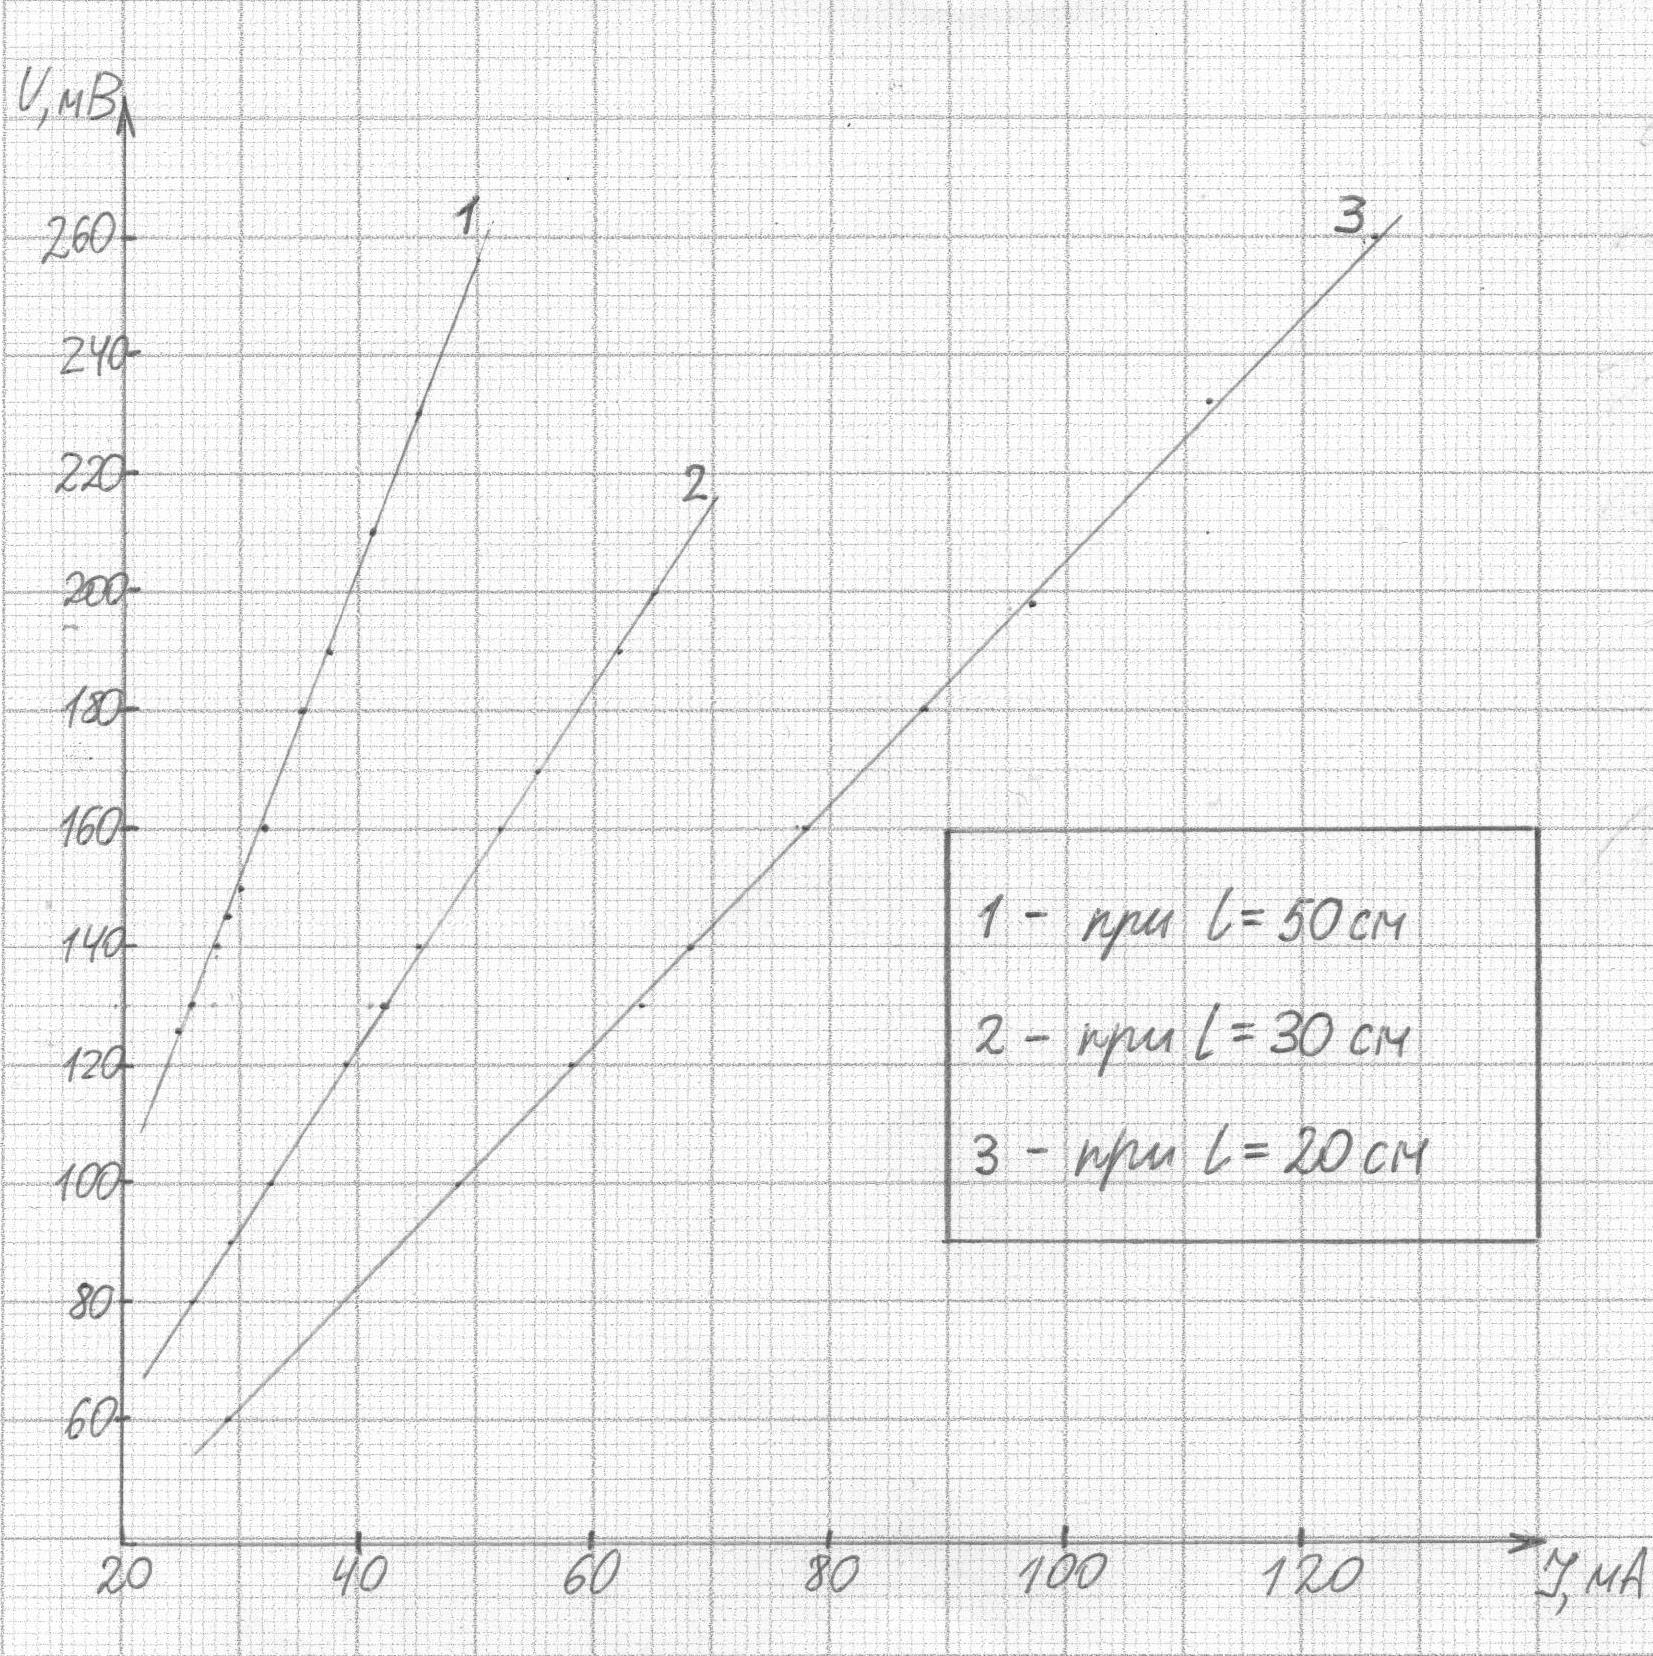
\includegraphics[width=0.55\linewidth]{plot.jpg}
		\caption{График зависимости U(I)}
		\label{fig:g}
	\end{figure}
	
	Графический метод определения R не подходит, т.к. погрешности измерений тока и напряжения малы и не могут быть отмечены на графике. Поэтому используем метод наименьших квадратов.
	
	
		
		\begin{tabular}{|c|c|c|} 
			\hline
			$UI$ & $I^{2}$ & $U^{2}$ \\
			\hline
			3341,0  & 660,49   & 16900 \\
			3878,0  & 767,29   & 19600 \\
			5072,0  & 1004,89  & 25600 \\
			7125,0  & 1406,25  & 36100 \\
			10396,0 & 2043,04  & 52900 \\
			8694,0  & 1713,96  & 44100 \\
			6354,0  & 1246,09  & 32400 \\
			4425,0  & 870,25   & 22500 \\
			4089,6  & 806,56   & 20736 \\
			3112,2  & 610,09   & 15876 \\
			\hline
			5648,68  & 1112,89  & 28671,20 \\
			\hline
		\end{tabular}
		\begin{tabular}{|c|c|c|}
			\hline
			$UI$ & $I^{2}$ & $U^{2}$ \\
			\hline
			5486  & 1780,84  & 16900 \\
			6356  & 2061,16  & 19600 \\
			9401  & 3058,09  & 28900 \\
			11780 & 3844,00  & 36100 \\
			13060 & 4264,09  & 40000 \\
			8320  & 2704,00  & 25600 \\
			4716  & 1544,49  & 14400 \\
			3270  & 1069,29  & 10000 \\
			2637  & 858,49   & 8100 \\
			2080  & 676,00   & 6400 \\
			\hline
			6710,60  & 2186,05  & 20600  \\
			\hline
		\end{tabular}
		\begin{tabular}{|c|c|c|}
			\hline
			$UI$ & $I^{2}$ & $U^{2}$ \\
			\hline
			8281,0  & 4057,69  & 16900 \\
			9534,0  & 4637,61  & 19600 \\
			15786,0 & 7691,29  & 32400 \\
			25737,0 & 12521,61 & 52900 \\
			32864,0 & 15976,96 & 67600 \\
			19186,2 & 9389,61  & 39204 \\
			12448,0 & 6052,84  & 25600 \\
			6984,0  & 3387,24  & 14400 \\
			4850,0 & 2352,25  & 10000 \\
			1752,0  & 852,64   & 3600\\
			\hline
			13742,22 & 6691,97  & 28220,4 \\
			\hline
		\end{tabular}
		\\
	
	
	Определим среднее значение R, случайную и систематическую погрешности по формулам:
	
	\begin{equation}
		\bar{R} = \frac{\langle UI \rangle}{\langle I^{2} \rangle}
	\end{equation}
	
	\begin{equation}
		\sigma_{r} = \frac{1}{\sqrt{10}} \sqrt{\frac{\langle U^{2} \rangle}{\langle I^{2} \rangle} - \bar{R}^{2}}
	\end{equation}
	
	\begin{equation}
		\sigma_{s} = \bar{R} \sqrt{(\frac{\sigma_{V}}{V})^{2}+(\frac{\sigma_{I}}{I})^{2}}
	\end{equation}
	
	
	Имеем:
	\begin{table}[htbp]
		\centering
		\begin{tabular}{c|ccc}
		$l$, см	&50          &30          &20  \\
		\hline
		$\langle R \rangle$, Ом	& 5,076    & 3,070    & 2,054 \\
		$\sigma_{r}$, Ом	& 0,005    & 0,003    & 0,002 \\
		$\sigma_{s}$, Ом	& 0,006    & 0,008    & 0,004 \\
		$\sigma$, Ом	& 0,008    & 0,008    & 0,004 \\
		\end{tabular}
	\end{table}
	
	Наносим на график прямые с полученными угловыми коэффициентами (рис. 2) и убеждаемся, что вычисления верны.
	
	
	
	Делаем поправку на неидеальный вольтметр:
	
	\begin{equation}
		R^{*} = R + \frac{R^{2}}{R_{V}}
	\end{equation}
	
	Имеем:
	
	\begin{equation}
		\fbox{$R_{50}=(5,089 \pm 0,008)$ Ом; $R_{30}=(3,075 \pm 0,008)$ Ом; $R_{20}=(2,056 \pm 0,004)$ Ом}		
	\end{equation}
	
	\subsection*{Удельное сопротивление}
	
	Для трёх опытов находим среднее значение удельного сопротивления по формуле (1) и погрешность по формуле:
	
	\begin{equation}
		\sigma_{\rho} = \rho \sqrt{(\frac{\sigma_{R}}{R})^{2}+(2\frac{\sigma_{d}}{d})^{2}+(\frac{\sigma_{l}}{l})^{2}}
	\end{equation}
	
	Подставив результаты (12) и (20)  во всех трёх случаях имеем:
	
	\begin{equation}
		\framebox{$\rho=(7,2 \pm 0,5) \cdot 10^{-7}$ Ом $\cdot$ м}
	\end{equation}
	
	Определим относительную погрешность:
	
	\begin{equation}
		\varepsilon_{\rho} = \frac{\sigma_{\rho}}{\rho} \cdot 100\% \approx 7\%
	\end{equation}
	
	
	\section*{Анализ результатов}
		
	Удельное сопротивление определено с относительной погрешностью 7\%. Наибольший вклад в ошибку даёт измерение диаметра проволоки (3,3\%), который в формуле (1) стоит во второй степени.
	
	Полученное значение $(0,67...0,77) \cdot 10^{-6}$ Ом $\cdot$ м меньше табличного $(1,05...1,40) \cdot 10^{-6}$ Ом $\cdot$ м.
	
	Можно предположить, что измеренный диаметр меньше реального. Действительно, форма и площадь поперечного сечения проволоки на самом деле непостоянны. В частности, ГОСТ Р ИСО 22034-2-2013 устанавливает разные допуски на диаметр проволоки 0,3 мм вплоть до 0,025 мм. Если подставить значение $d = 0,325$мм, получится среднее $\rho = 0,83 \cdot 10^{-6}$ Ом $\cdot$ м , что ближе к справочным данным.
	
	
	\section*{Заключение}
	Цели работы достигнуты: измерено удельное сопротивление нихромовой проволоки и вычислены систематические и случайные погрешности измерений. Все необходимые измерения проведены с достаточной точностью, кроме измерения диаметра проволоки. Результат работы не совпадает со справочными данными. Причины отклонения рассмотрены и связаны, прежде всего, с несовершенством проволоки и приборов и методов для измерения её диаметра.
	
	Важным и самым трудоёмким этапом работы было измерение сопротивления отрезка проволоки. Оно подтвердило теоретическую зависимость тока и напряжения, выражаемую законом Ома для участка цепи. Заметим, что благодаря большому числу измерений и применению точных методов анализа экспериментальных данных, а именно метода наименьших квадратов вместо графического, удалось достичь высокой точности измерения сопротивления, сравнимой с точностью моста постоянного тока.
	
	
	
	
\end {document}